%%%%%%%%%%%%%%%%%%%%%%%%%%%%%%%%%%%%%%%%%%%%%%%%%%%%%%%%%%%%%%%%%%%%%%%%
%%%%%%%%%%%%%%%%%%%%%% Simple LaTeX CV Template %%%%%%%%%%%%%%%%%%%%%%%%
%%%%%%%%%%%%%%%%%%%%%%%%%%%%%%%%%%%%%%%%%%%%%%%%%%%%%%%%%%%%%%%%%%%%%%%%

%%%%%%%%%%%%%%%%%%%%%%%%%%%%%%%%%%%%%%%%%%%%%%%%%%%%%%%%%%%%%%%%%%%%%%%%
%% NOTE: If you find that it says                                     %%
%%                                                                    %%
%%                           1 of ??                                  %%
%%                                                                    %%
%% at the bottom of your first page, this means that the AUX file     %%
%% was not available when you ran LaTeX on this source. Simply RERUN  %%
%% LaTeX to get the ``??'' replaced with the number of the last page  %%
%% of the document. The AUX file will be generated on the first run   %%
%% of LaTeX and used on the second run to fill in all of the          %%
%% references.                                                        %%
%%%%%%%%%%%%%%%%%%%%%%%%%%%%%%%%%%%%%%%%%%%%%%%%%%%%%%%%%%%%%%%%%%%%%%%%

%%%%%%%%%%%%%%%%%%%%%%%%%%%% Document Setup %%%%%%%%%%%%%%%%%%%%%%%%%%%%

% Don't like 10pt? Try 11pt or 12pt
\documentclass[10pt]{article}

% This is a helpful package that puts math inside length specifications
\usepackage{calc}
\usepackage[czech, english]{babel}
\usepackage[utf8]{inputenc}
\usepackage{graphicx}
\usepackage{comment}

\hyphenation{Android OpenVPN}

% Simpler bibsection for CV sections
% (thanks to natbib for inspiration)
\makeatletter
\newlength{\bibhang}
\setlength{\bibhang}{1em}
\newlength{\bibsep}
 {\@listi \global\bibsep\itemsep \global\advance\bibsep by\parsep}
\newenvironment{bibsection}
    {\minipage[t]{\linewidth}\list{}{%
        \setlength{\leftmargin}{\bibhang}%
        \setlength{\itemindent}{-\leftmargin}%
        \setlength{\itemsep}{\bibsep}%
        \setlength{\parsep}{\z@}%
        }}
    {\endlist\endminipage}
\makeatother

% Layout: Puts the section titles on left side of page
\reversemarginpar

%
%         PAPER SIZE, PAGE NUMBER, AND DOCUMENT LAYOUT NOTES:
%
% The next \usepackage line changes the layout for CV style section
% headings as marginal notes. It also sets up the paper size as either
% letter or A4. By default, letter was used. If A4 paper is desired,
% comment out the letterpaper lines and uncomment the a4paper lines.
%
% As you can see, the margin widths and section title widths can be
% easily adjusted.
%
% ALSO: Notice that the includefoot option can be commented OUT in order
% to put the PAGE NUMBER *IN* the bottom margin. This will make the
% effective text area larger.
%
% IF YOU WISH TO REMOVE THE ``of LASTPAGE'' next to each page number,
% see the note about the +LP and -LP lines below. Comment out the +LP
% and uncomment the -LP.
%
% IF YOU WISH TO REMOVE PAGE NUMBERS, be sure that the includefoot line
% is uncommented and ALSO uncomment the \pagestyle{empty} a few lines
% below.
%

%% Use these lines for letter-sized paper
% \usepackage[paper=letterpaper,
%             %includefoot, % Uncomment to put page number above margin
%             marginparwidth=1.2in,     % Length of section titles
%             marginparsep=.05in,       % Space between titles and text
%             margin=1in,               % 1 inch margins
%             includemp]{geometry}

%% Use these lines for A4-sized paper
\usepackage[paper=a4paper,
           %includefoot, % Uncomment to put page number above margin
           marginparwidth=25.5mm,    % Length of section titles
           marginparsep=1.5mm,       % Space between titles and text
           margin=20mm,              % 25mm margins
	   top=15mm,
           includemp]{geometry}

%% More layout: Get rid of indenting throughout entire document
\setlength{\parindent}{0in}

%% This gives us fun enumeration environments. compactitem will be nice.
\usepackage{paralist}

%% Reference the last page in the page number
%
% NOTE: comment the +LP line and uncomment the -LP line to have page
%       numbers without the ``of ##'' last page reference)
%
% NOTE: uncomment the \pagestyle{empty} line to get rid of all page
%       numbers (make sure includefoot is commented out above)
%
\usepackage{fancyhdr,lastpage}
% \usepackage{fancyhdr}
\pagestyle{fancy}
%\pagestyle{empty}      % Uncomment this to get rid of page numbers
\fancyhf{}\renewcommand{\headrulewidth}{0pt}
\fancyfootoffset{\marginparsep+\marginparwidth}
\newlength{\footpageshift}
\setlength{\footpageshift}
          {0.5\textwidth+0.5\marginparsep+0.5\marginparwidth-2in}
\lfoot{\hspace{\footpageshift}%
       \parbox{4in}{\, \hfill %
                     \arabic{page} z \protect\pageref*{LastPage} % +LP
%                    \arabic{page}                               % -LP
                    \hfill \,}}

% Finally, give us PDF bookmarks
\usepackage{color,hyperref}
\definecolor{darkblue}{rgb}{0.0,0.0,0.3}
\hypersetup{colorlinks,breaklinks,
            linkcolor=darkblue,urlcolor=darkblue,
            anchorcolor=darkblue,citecolor=darkblue}

%%%%%%%%%%%%%%%%%%%%%%%% End Document Setup %%%%%%%%%%%%%%%%%%%%%%%%%%%%


%%%%%%%%%%%%%%%%%%%%%%%%%%% Helper Commands %%%%%%%%%%%%%%%%%%%%%%%%%%%%

% The title (name) with a horizontal rule under it
%
% Usage: \makeheading{name}
%
% Place at top of document. It should be the first thing.
\newcommand{\makeheading}[1]%
        {\hspace*{-\marginparsep minus \marginparwidth}% 
         \begin{minipage}[t]{\textwidth+\marginparwidth+\marginparsep}%		
% 		\centering{\Large \textit{Curriculum Vitae} } \\[0.5cm] % Added Curriculum Vitae heading
                {\LARGE \bfseries #1 \hfill   
		 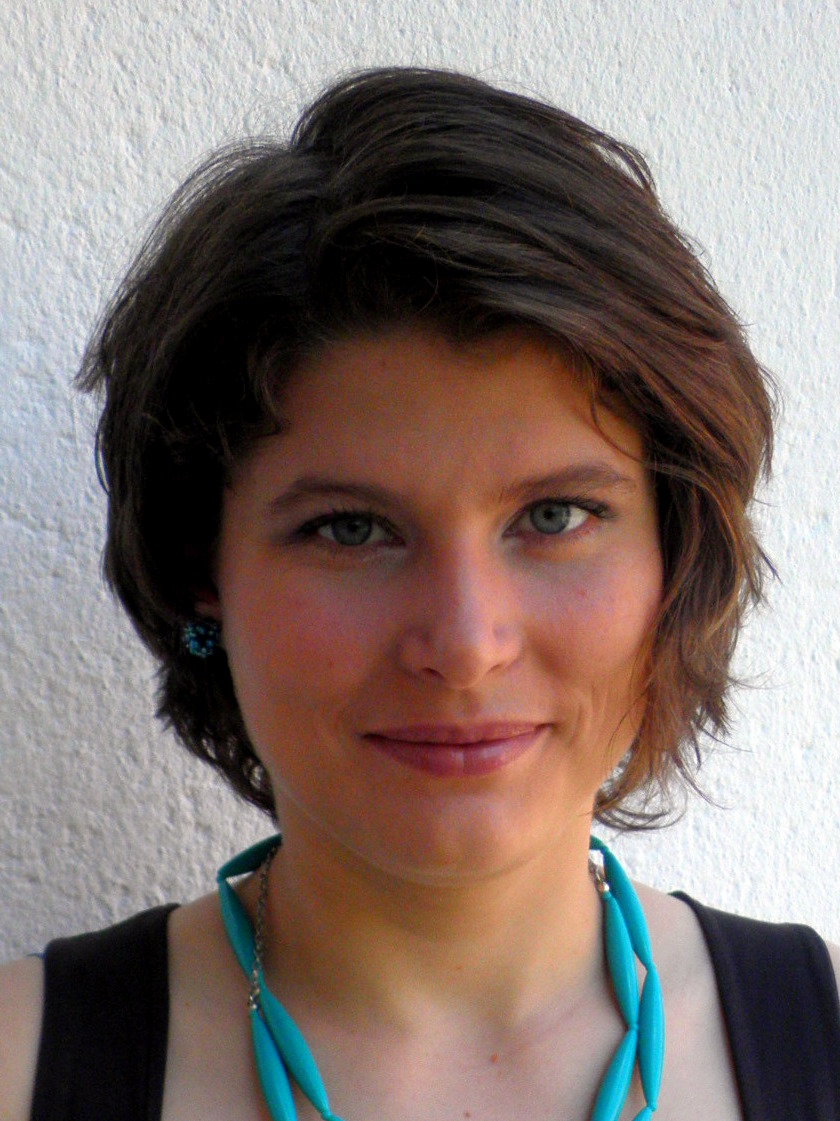
\includegraphics[width=2cm]{foto1} % Added photo
		}\\[-0.15\baselineskip]%
                 \rule{\columnwidth}{1pt}%
         \end{minipage}}

% The section headings
%
% Usage: \section{section name}
%
% Follow this section IMMEDIATELY with the first line of the section
% text. Do not put whitespace in between. That is, do this:
%
%       \section{My Information}
%       Here is my information.
%
% and NOT this:
%
%       \section{My Information}
%
%       Here is my information.
%
% Otherwise the top of the section header will not line up with the top
% of the section. Of course, using a single comment character (%) on
% empty lines allows for the function of the first example with the
% readability of the second example.
\renewcommand{\section}[2]%
        {\pagebreak[2]\vspace{1.3\baselineskip}%
         \phantomsection\addcontentsline{toc}{section}{#1}%
         \hspace{0in}%
         \marginpar{
         \raggedright \scshape #1}#2}

% An itemize-style list with lots of space between items
\newenvironment{outerlist}[0]%
        {\begin{itemize}}
	{\end{itemize}
         \vspace{-.6\baselineskip}}

% An environment IDENTICAL to outerlist that has better pre-list spacing
% when used as the first thing in a \section
\newenvironment{lonelist}[1][\enskip\textbullet]
        {\vspace{-\baselineskip}\begin{list}{#1}{
        \setlength{\partopsep}{0pt}
        \setlength{\topsep}{0pt}}}
        {\end{list}\vspace{-.6\baselineskip}}

% An itemize-style list with little space between items
\newenvironment{innerlist}[0]%
        {\begin{compactitem}}
	{\end{compactitem}}

% To add some paragraph space between lines.
% This also tells LaTeX to preferably break a page on one of these gaps
% if there is a needed pagebreak nearby.
\newcommand{\blankline}{\quad\pagebreak[2]}
%
\renewcommand{\labelitemii}{\textbullet}
%

%%%%%%%%%%%%%%%%%%%%%%%% End Helper Commands %%%%%%%%%%%%%%%%%%%%%%%%%%%

%%%%%%%%%%%%%%%%%%%%%%%%% Begin CV Document %%%%%%%%%%%%%%%%%%%%%%%%%%%%

\begin{document}

% \begin{minipage}[t]{\textwidth+\marginparwidth+\marginparsep}
% \centering{\LARGE \textit{Curriculum Vitae} } \\
% 
% \end{minipage}



% \setlength\fboxsep{0pt}
% \setlength\fboxrule{0pt}
% \fbox{\includegraphics[width=60px,height=90px]{mahnamahna90}}


\makeheading{Lenka Křivánková}


\section{Osobní údaje}
%
% NOTE: Mind where the & separators and \\ breaks are in the following
%       table.
%
% ALSO: \rcollength is the width of the right column of the table
%       (adjust it to your liking; default is 1.85in).
%
\newlength{\rcollength}\setlength{\rcollength}{2.5in}%
%
\begin{tabular}[t]{@{}p{\textwidth-\rcollength}p{\rcollength}}
\textit{Datum narození:} 31. 10. 1984 		& \textit{Mobil:} +420 777 618 329 \\
\textit{Adresa:} Bezručova 14, Brno 602 00         	& \textit{E-mail:} \href{mailto:lenka.krivankova@email.cz}{lenka.krivankova@email.cz}\\
%60200 Czech Republic    & \textit{Web:} \href{http://ondrejcermak.info/}{ondrejcermak.info}\\
\end{tabular}

% \section{Citizenship}
%% 
% Czech Republic

%\section{Objective}
% 
%Software Engineering role focusing on smartphone and internet technologies.

%%%%%%%%%%%%%%%%%%%%%%%%%%

\section{Vzdělání}
%
\href{http://muni.cz/}{\textbf{Masarykova Univerzita}},
	  \href{http://sci.muni.cz}
	      {Přírodovědecká fakulta},
Brno

\begin{outerlist}
   \item[] 2009 - dosud\ \textbf{Doktorský studijní program: Matematika},
	  \begin{innerlist}
	    \item[] Obor: Pravděpodobnost, statistika a matematické modelování
	    \item Závěrečná práce: \emph{Stochastické metody analýzy ekonomických dat} \hfill \\
	  \end{innerlist}

  \item[] 2007 - 2009\ \textbf{Magisterský studijní program: Aplikovaná matematika},
	  \begin{innerlist}
	    \item[] Obor: Statistika a analýza dat
	    \item Závěrečná práce: \emph{Wienerův proces a jeho aplikace} \hfill \\
             \end{innerlist}

  \item[] 2004 - 2007\ \textbf{Bakalářský studijní program: Aplikovaná matematika},
	  \begin{innerlist}
	    \item[] Obor: Statistika a analýza dat
               \item[] Obor: Finanční a pojistná matematika	    
               \item Závěrečná práce: \emph{Stochastické procesy ve finanční matematice} \hfill \\
             \end{innerlist}

%  \item[] \textbf{Bachelor's degree},
%	  \href{http://fel.cvut.cz}
%	      {Faculty of Electrical Engineering},\\
%	      09/2006 - 09/2009
%	  \begin{innerlist}
%	    \item \emph{cum laude}, with praise	    
%	    \item Scholarships for excellence granted repeatedly during the studies
%	    \item Specialization: Information Technology
%	    \item Thesis topic: \emph{Application Mantichora - Scene Editor} \hfill \\
%	    Analysis and implementation of scene format and 3D scene editor for space simulator using Java3D and XML.
%	  \end{innerlist}
\end{outerlist}

\blankline

\href{http://www.jaroska.cz/}{\textbf{Gymnázium Brno, třída Kapitána Jaroše}}

\begin{outerlist}
  \item[]  2000 - 2004\ zaměření na matematiku
\end{outerlist}

%%%%%%%%%%%%%%%%%%%%%%%%%%

\section{Publikační činnost}
%
KAFKOVÁ, Silvie, Lenka KŘIVÁNKOVÁ a Marie LEVÁKOVÁ.  \href{https://www.muni.cz/vyzkum/publikace/1167343}
	      {Survival analysis of patients with brain tumour}. In Jiří Zelinka, Martin Řezáč. {\it Mathematical
Models and Financial Mathematics, Book of short papers.} Brno: Masaryk University, 2014. s. 27--33, 7 s. ISBN 978-80-210-6648-9.

KŘIVÁNKOVÁ, Lenka.  \href{http://www.muni.cz/research/publications/1093598}
	      {Asset-Pricing Models in Portfolio Theory}. In Jiří Zelinka, Martin Řezáč. {\it Financial Mathematics in Practice II, Book of short papers.} Brno: Masaryk University, 2013. s. 42-49, 8 s. ISBN 978-80-210-6176-7.

KŘIVÁNKOVÁ, Lenka. \href{http://www.muni.cz/research/publications/1077842}
	      {Continuous-Time Models in Portfolio Theory}. In  {\it XX International Conference PDMU-2012 Problems of Decision Making under Uncertainties.} Brno: University of Defence, 2012. s. 95-104, 10 s. ISBN 978-80-7231-897-1.

KAFKOVÁ, Silvie a Lenka KŘIVÁNKOVÁ.  \href{http://www.muni.cz/research/publications/976825}
	      {The Vasicek Model and Estimation of its Parameters}. In  {\it Workshop of the Jaroslav Hájek Center and Financial Mathematics in Practice I, Book of short papers.} Brno: Masaryk University, 2012. s. 24-29, 6 s. ISBN 978-80-210-5778-4.

KŘIVÁNKOVÁ, Lenka.  \href{http://www.muni.cz/research/publications/979237}
	      {The Black-Scholes equation for barrier options}. In  {\it 7. konference o matematice a fyzice na vysokých školách technických s mezinárodní účastí : Sborník příspěvků část 1 - matematika.} 2011. 8 s. ISBN 978-80-7231-815-5.

KŘIVÁNKOVÁ, Lenka. \href{http://www.muni.cz/research/publications/979245}
	      {Wiener process and applications}. In  {\it Workshop of the Jaroslav Hájek Center, Book of short papers.} 2010. 4 s. ISBN 978-80-210-5100-3.

KŘIVÁNKOVÁ, Lenka a Martin KOLÁŘ. \href{https://www.math.muni.cz/~vondra/uvm/vystupy/KA2/MF003/MF003.pdf}
	      {Oceňování finančních derivátů}. 2009.

%%%%%%%%%%%%%%%%%%%%%%%%%%

\section{Konference}
%
%\begin{outerlist}
\vspace{-20pt}
\begin{description}
  \item[09/2013] {Workshop Mathemetical Models and Workshop Financial Mathematics} 
  \item[05/2013] {International Student Conference on Applied Mathematics and Informatics}	  
  \item[09/2012] {Workshop Financial Mathematics in Practice II} 
  \item[09/2012] {XX International Conference PDMU-2012 Problems of Decision Making under Uncertainties} 
  \item[09/2011] {Workshop of the Jaroslav Hájek Center and Workshop Financial Mathematics in Practice I} 
  \item[09/2011] {7.~konference o matematice a fyzice na vysokých školách technických s mezinárodní účastí} 
  \item[09/2010] {Workshop of the Jaroslav Hájek Center} 
  \item[09/2009] {Workshop of the Jaroslav Hájek Center} 
\end{description}

%%%%%%%%%%%%%%%%%%%%%%%%%%

\section{Kurzy}
%
%\begin{outerlist}
\vspace{-20pt}
\begin{description}
  \item[04/2017] {R školení} 
  \item[01/2013] {SAS pro Masarykovu univerzitu} 
  \item[11/2012] {Seminář prezentačních dovedností}	  
  \item[09/2012] {Data mining v softwaru STATISTICA 10} 
  \item[06/2012] {Bayesian Analysis with R and WinBUGs} 
%  \item {SAS pro Masarykovu univerzitu} ,
%{Seminář prezentačních dovedností},	  
%  \item {Data mining v softwaru STATISTICA 10}, 
%{Bayesian Analysis with R and WinBUGs} 
\end{description}
%\end{outerlist}

%%%%%%%%%%%%%%%%%%%%%%%%%%

\section{Výuka}
%
\href{http://muni.cz/}{\textbf{Masarykova Univerzita}},
	  \href{http://econ.muni.cz}
	      {Ekonomicko-správní fakulta},
%	  \href{http://www.econ.muni.cz/katedra-aplikovane-matematiky-a-informatiky/}
%	      {Katedra aplikované matematiky a informatiky},
Brno
\begin{outerlist}
  \item[] \textit{Externí vyučující} 
	  \hfill \textbf{02 - 06/2013}
  \begin{innerlist}    
    \item cvičení předmětu Statistika 2; příprava; zkoušení
  \end{innerlist}
\end{outerlist}

\blankline

\href{http://mendelu.cz/}{\textbf{Mendlova Univerzita}},
	  \href{http://www.pef.mendelu.cz/}
	      {Provozně ekonomická fakulta},
%	  \href{http://uso.pef.mendelu.cz/}
%	      {Ústav statistiky a operačního výzkumu},
Brno
\begin{outerlist}
  \item[] \textit{Technik pro výuku} 
	  \hfill \textbf{09/2010 - 12/2013}
  \begin{innerlist}    
    \item cvičení předmětů Statistika, Ekonometrie, Statistické zpracování dat;  zkoušení
    \item oponování závěrečných prací, administrativní práce
  \end{innerlist}
\end{outerlist}

%%%%%%%%%%%%%%%%%%%%%%%%%%%

\section{Praxe}
%
\href{http://www.sberbankcz.cz/}{\textbf{Sberbank}}, {oddělení Integrated Risk Management},
Brno
\begin{outerlist}
  \item[] \textit{Risk Analyst, team leader} 
	  \hfill \textbf{11/2014 - dosud}
  \begin{innerlist}    
    \item vedení týmu Reporting, Analytics and Local Models
    \item implementace nových požadavků na reporting
    \item řízení procesu výpočtu opravných položek (technicky i metodicky)
  \end{innerlist}
  \item[] \textit{Credit Risk Analyst} 
	  \hfill \textbf{08/2013 - 10/2014}
  \begin{innerlist}    
    \item credit risk reporting, regulatorní reporting 
    \item alokace zajištění, výpočet opravných položek
  \end{innerlist}
\end{outerlist}

\blankline

\href{http://muni.cz/}{\textbf{Masarykova Univerzita}},
	  \href{http://www.muni.cz/ics}
	      {Ústav výpočetní techniky},
Brno
\begin{outerlist}
  \item[] \textit{Administrátorka OPVK projektu}
	  \hfill \textbf{08 - 11/2012}
  \begin{innerlist}    
    \item projekt Standardizace IT gramotnosti na Masarykově univerzitě (SITMU)
    \item vedení administrativy projektu, příprava monitorovací zprávy, komunikace s řešiteli
  \end{innerlist}
\end{outerlist}

%%%%%%%%%%%%%%%%%%%%%%%%%%

\section{Počítačové znalosti}
%
\vspace{-20pt}
\begin{description}
\item[Operační systémy] MS Windows (uživatelská znalost), Linux (uživatelská znalost)
\item[Kancelářské programy] MS Word, MS Excel, MS PowerPoint, IBM Notes, \TeX
\item[Matematické programy] STATISTICA, R, WinBUGs, Maple, Matlab, SAS
\item[Ostatní] SQL, Pascal, Inkscape, Google Apps
\end{description}

\section{Ostatní}
%
\vspace{-20pt}
\begin{description}
\item[Řidičský průkaz] B (aktivní řidič)
\item[Zájmy] skauting (vedoucí), matematika a statistika, šifrovací hry, volejbal, lyžování
\end{description}

\end{document}

%%%%%%%%%%%%%%%%%%%%%%%%%% End CV Document %%%%%%%%%%%%%%%%%%%%%%%%%%%%%
